\chapter{Egy frekvenciaváltó tervezése}

\paragraph{}
Tesla 1888-ban bemutatott három fázisú indukciós motorjával, nyilvánvalóvá vált, hogy az ilyen típusú gépek megbízhatóbbak és gazdaságosabbak tudnak lenni, mint az egyenáramú társaik. Jelentős hátrányuk azonban, hogy a vezérlésükhöz három fázisú feszültséget kell előállítani, mely akkoriban csak egy szintén három fázisú generátor segítségével volt megoldható. Manapság a három fázisú teljesítmény a villamos hálózatnak köszönhetően rendelkezésre áll, azonban még így is vet fel problémákat ezen motorok üzemeltetése.

\paragraph{}
A frekvenciaváltó egy olyan eszköz mely váltakozó áramú bemenetből váltakozó áramú kimenetet állít elő, mint ahogy a neve is mutatja, más frekvenciával vagy akár feszültséggel, mint a bemenet. Erre azért van szükség, mert a meghajtani kívánt folyamatnak nagyon valószínű, hogy más igényei vannak, mint amit a hálózat önmagában képes biztosítani. Értem ez alatt azt, hogy közvetlen összeköttetés esetén a motorunk $50\ Hz$-el, vagy ennek egész számú hányadosával tudna forogni, illetve ennek a paraméter a befolyásolása csak a motor fizikai módosításával lehetséges, azaz más pólus pár számú motort kell beépíteni. Természetesen mint az ipar és az élet minden szegmensében itt is célunk a feladat minél hatékonyabb végrehajtása. A világon a teljes villamosenergia felhasználás mint egy $25\ \%$-át adják a villamos hajtások és ez a szám folyamatosan nő (például az elektromos közlekedés tér nyerésével). Az igény tehát nyilvánvaló ezen eszközöknek folyamatos fejlesztésére.

\begin{figure}[!h]
	\centering
	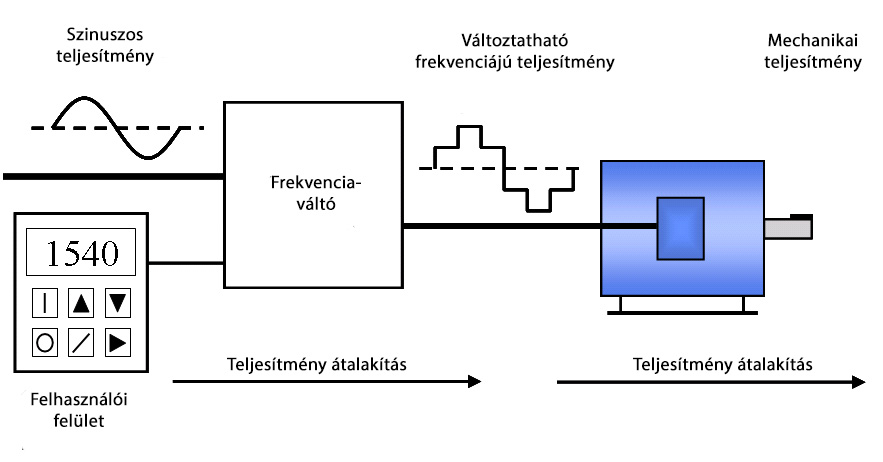
\includegraphics[width = 0.8\textwidth]{figures/VFD_System.jpg}
	\caption{A frekvenciaváltó szerepe} 
	\label{fig:vfd_system}
\end{figure}

\paragraph{}
Az eszköz feladatát jól összefoglalja \aref{fig:vfd_system} ábra. A hálózatból érkező teljesítményt, a felhasználó által megadott paraméterekkel átalakítjuk, majd a terhelő gépet meghajtjuk vele. A modern hajtások azért ennél már jóval szofisztikáltabb működésre is képesek, gondoljunk itt akár táv felügyeletre, identifikációra, vagy esetleg akár vezeték nélküli hozzáférésre. Szükség lehet konstans fordulatszám, vagy konstans nyomaték tartásra, esetleg pontos pozíció szabályozásra. Más igények mutatkoznak egy szállító szalag, egy víz pumpa, vagy egy szellőztető ventilátor esetén.

\paragraph{}
A korábban az ilyen teljesítmény átalakítási feladatokat elektromechanikus berendezésekkel oldották meg, nevezetesen egy motor és generátor párral, ahol is a megfelelő pólus pár arány kiválasztásával a frekvenciát módosítani lehetett. Amennyiben szükséges volt feszültség módosítás is, megfelelő áttételű transzformátor segítségével valósították meg. Ennek a megoldásnak hátránya a nagy teljesítmény esetén nagy méretű villamos gép, ennek megfelelően a kicsi teljesítmény-sűrűség. A megbízhatóságot csökkenti a mozgó alkatrészek jelenléte és folyamatos igénybevétele, illetve a nagy forgó tömeg is hordoz magában veszélyeket. Ezt követően megjelentek a vákumcsöves eszközök, azonban az igazi áttörést a teljesítmény-elektronikai félvezető elemek megjelenése okozta.

\paragraph{}
Ezek a modern eszközök már nem tartalmaznak mozgó alkatrészt (feltéve persze, hogy a reléket és kontaktorokat nem számítjuk mozgó alkatrésznek). A félvezető technológia fejlődésével egyre nagyobb és nagyobb teljesítmény-sűrűségeket tudunk elérni. A jövőben nagy lehetőség rejlik a $SiC \ - $  szilícium-karbid alapú félvezető eszközök használatában. Ezen típusú eszközök a napjainkban szokásosnál sokkal nagyobb kapcsolási frekvenciát is megengednek, így jelentősen csökkentető a beépített mágneses anyag tömege, ezáltal az eszköz mérete is. A FET-eken a maradék feszültség értéke is sokkal kisebb, mint az IGBT-ken, így a kapcsolási veszteség is kisebb lehet a nagyobb kapcsolási frekvencia ellenére. A $SiC$ alapú felvezetők sokkal magasabb hőmérsékleten is üzem képesek tudnak maradni, akár $200 °C$ körüli üzemi hőmérséklet is elérhető, aminek köszönhetően a hűtés hatékonyabbá válik, mivel a hűtő közeg és az eszköz között nagyobb lesz a $\Delata{}T$ hőmérséklet különbség. A mi frekvanciaváltóinkban még IGBT-k találhatóak, de a technológia fejlődésével a jövőben előfordulhat $SiC$ alapú frekvenciaváltó készítése is.

\begin{figure}[!h]
	\centering
	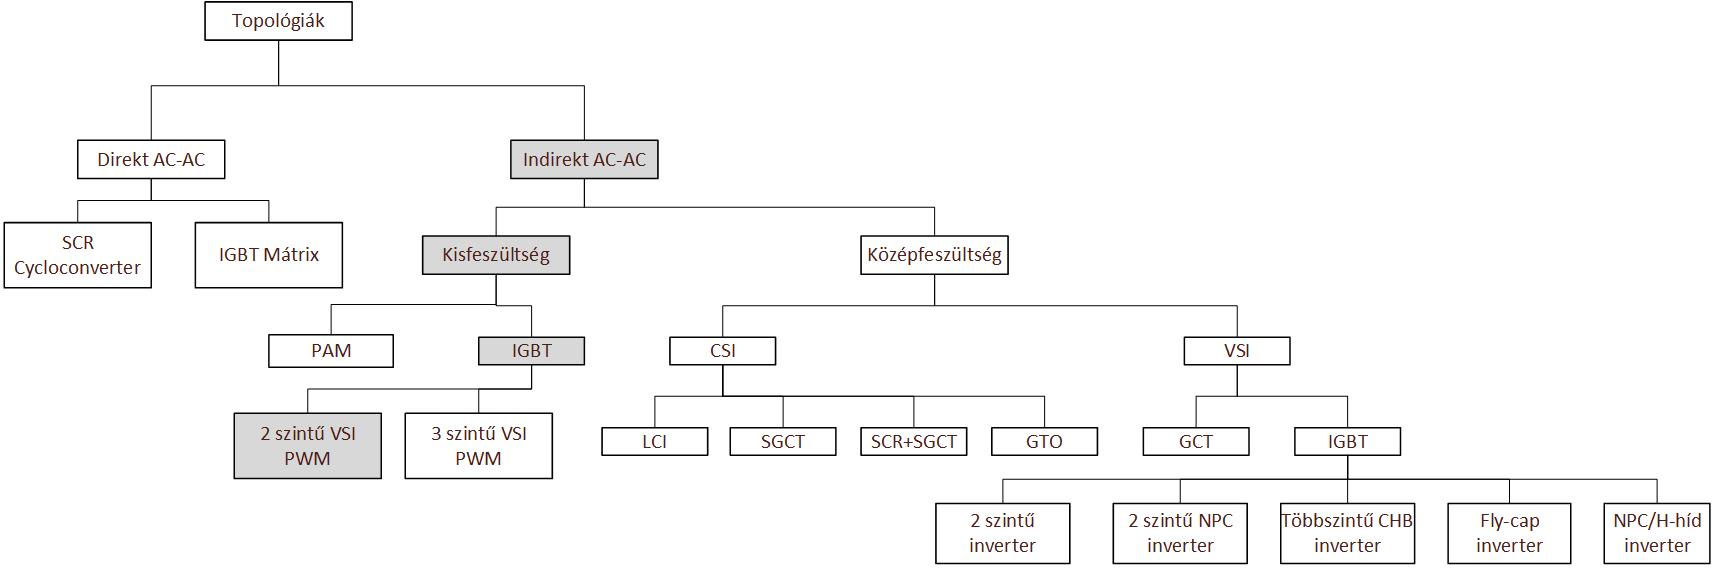
\includegraphics[width = \textwidth]{figures/topologies.jpg}
	\caption{A frekvenciaváltó típusok \cite{drivetypes}} 
	\label{fig:topologies}
\end{figure}

\Aref{fig:topologies} ábrán láthatjuk a napjainkban elterjedt inverter típusokat. Az ábrában szürkével kiemeltem a Hyundai által fejlesztett típust.

\section{Termék specifikáció}

A Hyundai által jelenleg fejlesztett frekvenciaváltó család kis feszültségű, általános célú PWM vezérlet IGBT kapcsoló elemű 2 szintű inverteres frekvenciaváltó, passzív front-end-el, azaz a hálózatra nem tud visszatáplálni. \Aref{fig:family} táblázatban látható a jelenleg fejlesztett termék család. \todo{wikipédia hivatkozás}

\begin{table}[]
\centering
\begin{tabular}{|c|c|c|c|l}
\cline{1-4}
\textbf{Név} & \textbf{Teljesítmény (kW)} & \textbf{Áram (A)} & \textbf{Tömeg (kg)} &  \\ \cline{1-4}
\multirow{4}{*}{\textbf{FR1}} & 0,55 & 3,7 & \multirow{4}{*}{6} &  \\ \cline{2-3}
 & 0,75 & 4,8 &  &  \\ \cline{2-3}
 & 1,1 & 6,6 &  &  \\ \cline{2-3}
 & 1,5 & 8 &  &  \\ \cline{1-4}
\multirow{3}{*}{\textbf{FR2}} & 2,2 & 11 & \multirow{3}{*}{10} &  \\ \cline{2-3}
 & 3,7 & 18 &  &  \\ \cline{2-3}
 & 5,5 & 25 &  &  \\ \cline{1-4}
\multirow{2}{*}{\textbf{FR3}} & 7,5 & 31 & \multirow{2}{*}{20} &  \\ \cline{2-3}
 & 11 & 48 &  &  \\ \cline{1-4}
\multirow{3}{*}{\textbf{FR4}} & 15 & 62 & \multirow{3}{*}{37,5} &  \\ \cline{2-3}
 & 18,5 & 75 &  &  \\ \cline{2-3}
 & 22 & 88 &  &  \\ \cline{1-4}
\multirow{3}{*}{\textbf{FR5}} & 30 & 114 & \multirow{3}{*}{66} &  \\ \cline{2-3}
 & 37 & 140 &  &  \\ \cline{2-3}
 & 45 & 170 &  &  \\ \cline{1-4}
\multirow{2}{*}{\textbf{FR6}} & 55 & 211 & \multirow{2}{*}{108} &  \\ \cline{2-3}
 & 75 & 261 &  &  \\ \cline{1-4}
\end{tabular}
\caption{A fejlesztés alatt álló termékpaletta}
\label{fig:family}
\end{table}

\paragraph{}
Azt, hogy a termék milyen széles területét lefedi az iparnak, jól jellemzi, hogy az ezt leíró dokumentum 52 különböző tételt különböztet meg. A teljesség igénye nélkül a felvevő piac néhány szelete:

\begin{itemize}
	\item{Nagyfeszültségű légkondícionálók}
	\item{Élelmiszeripar}
	\item{Textilipar}
	\item{Szállító szalagok}
	\item{Csomagolás és cimkézés}
	\item{Nyomtatás}
	\item{Gépi megmunkálás}
	\item{Autóipar}
\end{itemize}

\paragraph{}
A hardveres funkcionalitás nagyjából megegyezik minden esetben, az igazán nagy különbség az egyes területek között a szoftver funkcionalitásában van. Egy szállítószalag esetében fontos a pontos fordulatszám tartása, vagy a pontos pozíció beállítása, míg más felhasználás esetében a pontos nyomaték szabályozás lehet fontos, ilyen lehet például a villamos vontatás.

\paragraph{}
Amennyiben külön nincsen jelölve, a dolgozat a továbbiakban az FR1 (Frame 1) kódjelű, legkisebb frekvenciaváltóra hivatkozik a példák esetében.

\section{Az eszköz felépítése}

\paragraph{}
A frekvenciaváltó egyenirányítja a bejövő hálózati feszültséget, egy köztes energia tárolóban, az úgynevezett \emph{DC-link} kondenzátorban tárol némi energiát, hogy a feszültség lengését alacsonyan tartsa, majd egy kimeneti inverterrel előállítja a szükséges jel alakot. Ezt a vázlatot láthatjuk \aref{fig:vfd_schema} ábrán, kiemelve a hálózatot modellező ellenállást és induktivitást.

\begin{figure}[h]
	\centering
	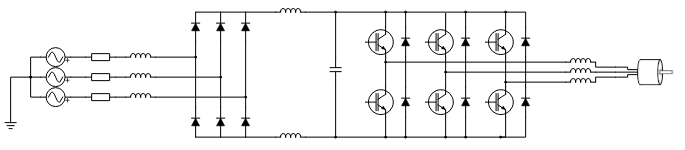
\includegraphics[width = \textwidth]{figures/VFDschematic_choke.png}
	\caption{A frekvenciaváltó egyszerű felépítése} 
	\label{fig:vfd_schema}
\end{figure}

\paragraph{}
Itt természetesen csak egy vázlatos ábrázolás látató, ezen nem szerepelnek a meghajató elektronikák, a vezérlés, a mérések, és még sok más. Jól látható azonban, hogy a folyamatra egyedül a félhidak vezérlésével tudunk hatni. A Frame 1-ben a kimeneti IGBT-k és diódák egy tokban vannak, egy Semikron SKiiP 24NAB12T4V1 modulban.

\section{A DC fojtó szerepe}

A frekvenciaváltók bemeneti fokozatára vagy DC vagy AC oldalon szokásos fojtót alkalmazni. Enélkül a DC kondenzátor, mint kis impedanciás terhelés jelenne meg a hálózat felé. Ha felteszünk egy ipari környezetben szokásos $1,6\ MVA$-s hálózatot, egyértelművé válik, hogy a hálózatból nagyságrendekkel nagyobb áramot ki tudunk venni, mint a frekvenciaváltó üzemi értékei, ebből adódóan a kondenzátor minden kommutációnál óriási áram tüskékkel töltődne. Az induktivitás ezeket a tüskéket simítja el, csökkentve a DC kondenzátort érő áram hullámosságot és a feszültség hullámosságot is. \Aref{fig:chokenochoke}. ábrán látható egy DC fojtóval ellátott és egy anélküli szimuláció eredménye. Látható, hogy a fojtóval ellátott esetben jelentősen kisebb a DC hullámosság, valamint az áram jelalakja is sokkal simább.

\begin{figure}[H!]
	\centering
	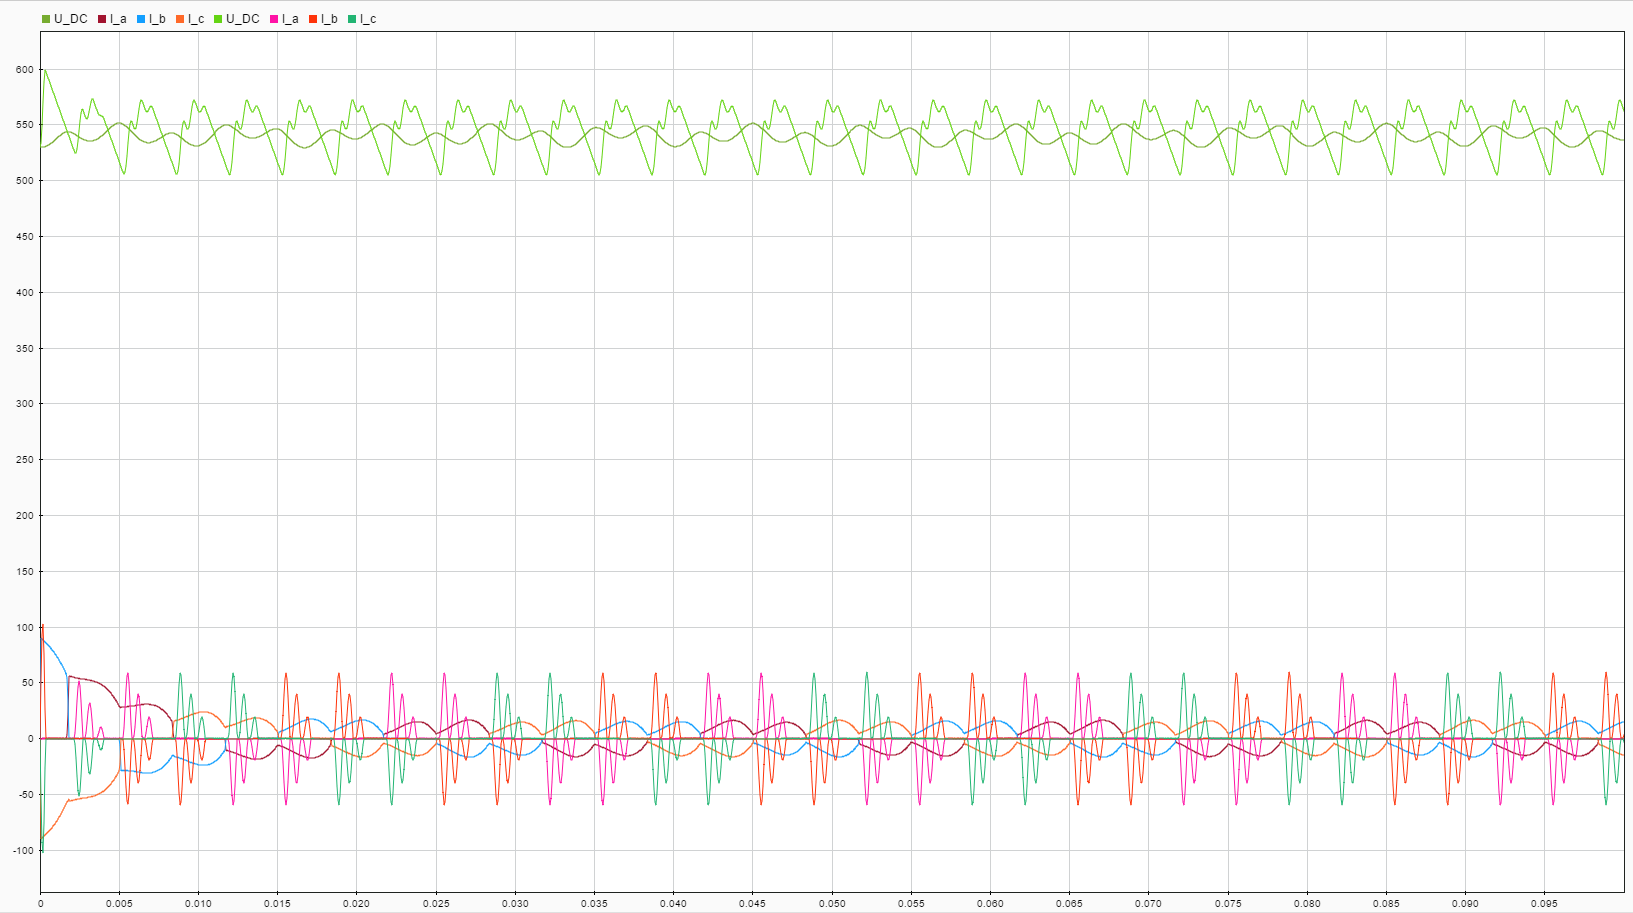
\includegraphics[width = \textwidth]{figures/choke_vs_nochoke_11A.png}
	\caption{A DC fojtó szerepe} 
	\label{fig:chokenochoke}
\end{figure}



\section{A szükséges kompetenciák}

A felépítés alapján elmondható, hogy egy ilyen termék összeállítása nagyon bonyolult feladat, sok területet lefed, sok féle kompetenciára van szükség. A teljesítmény elektronikai elemek és kapcsolálsok megtervezése gyakorlatilag csak az első gondolat. Ezen túl szükséges még a termikus méretezés, a vezérlő elektronikák tervezése, a különböző mérések megvalósítása. Amikor már ezzel is készen vagyunk, akkor a frekvenciaváltó tervezése elektronikai szempontból késznek mondható. Nem szabad megfeledkezni azonban arról, hogy ez egy készülék, melynek a mechanikus felépítéséről is gondoskodni kell. Itt kerülnek képbe a konstrukcióval foglalkozó gépész kollégák.

\begin{figure}[h]
	\centering
	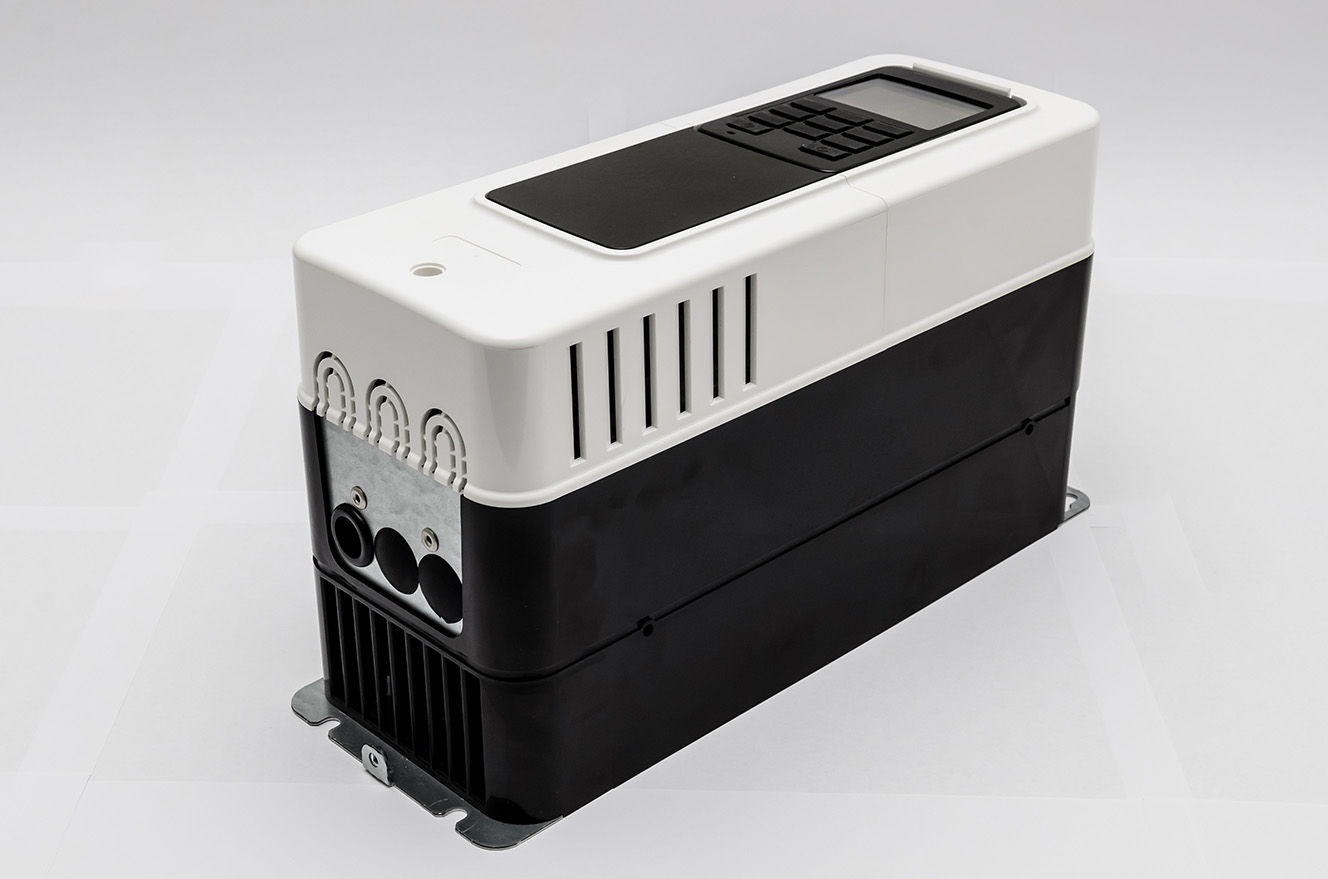
\includegraphics[width = 0.8\textwidth]{figures/n700_proto.jpg}
	\caption{Az elkészült Frame 1 prototípus} 
	\label{fig:n700_proto}
\end{figure}

\paragraph{}
A feladat már eddig is kellőképpen összetett volt, de a termékünk még mindig nem működő képes. Hiányzik belőle a szoftver, mely önmagában nagyon szerteágazó munka. Először is elő kell állítani a megfelelő szabályzókat, melyek segítségével elő tudunk állítani szinuszos kimenetet, gondoskodni kell a kapcsoló elemek vezérlő jelének megfelelő modulációjáról. Foglalkozni kell a magasabb szintű funkcionalitás megvalósításával, a különböző kommunikációs vonalak kezelésével, magának a rendszernek a menedzselésével. A HMI\footnote{Human-Machine Interface}-n is meg kell jelenteni információt, biztosítani kell lehetőséget a beavatkozásra. Amennyiben úgy gondolná az olvasó, hogy ez még nem annyira bonyolult, akkor figyelmébe ajánlom a PC-s szoftvert, melyet szintén különös gonddal el kell készíteni, ha egy jól használható terméket kívánunk előállatni, hiszen a felhasználó ezen keresztül fogja a legkönnyebben felkonfigurálni igényei szerint az eszközt.

\todo[inline]{Félbehagyott gondolat}

\begin{figure}[h]
	\centering
	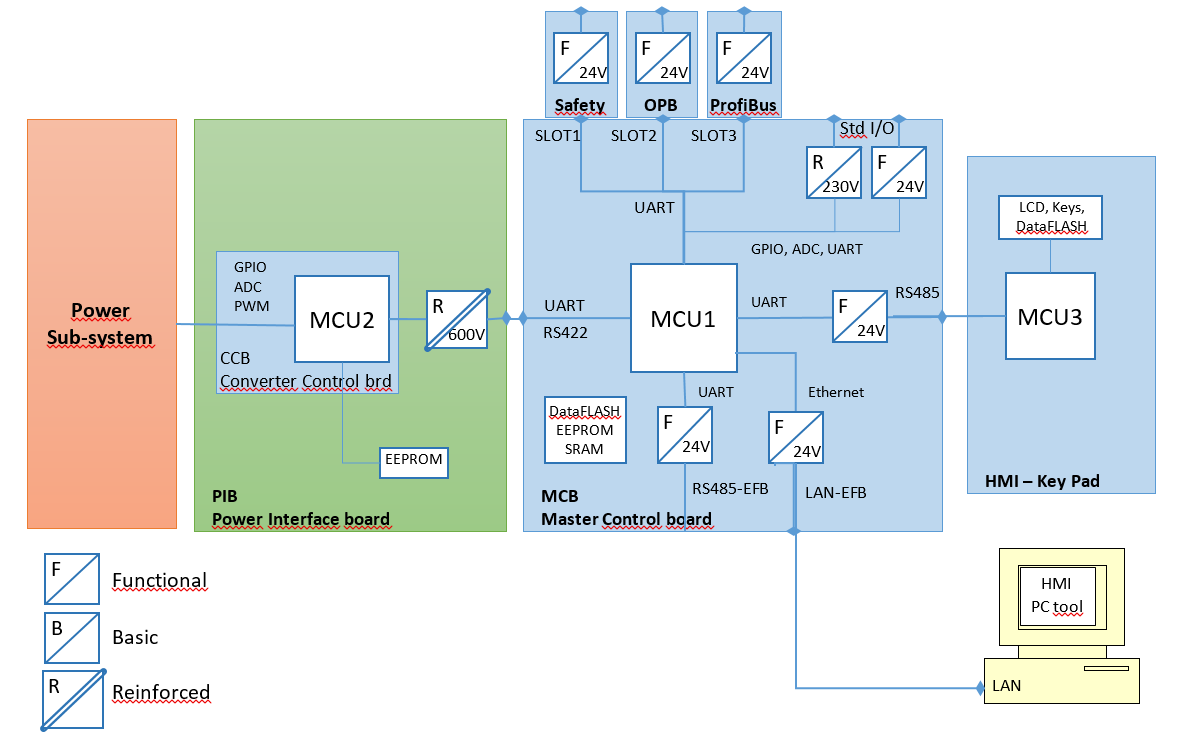
\includegraphics[width = \textwidth]{figures/architect.png}
	\caption{A vezérlő elektronika blokkvázlata} 
	\label{fig:hw_architect}
\end{figure}

\paragraph{}
\Afigref{hw_architect} ábrán látható a különböző elemek kapcsolata, illetve a kommunikáció közöttük. A CCB feladata a teljesítmény átalakítás közvetlen irányítása. Ez a kártya végzi az analóg méréseket, és ezen mérések, illetve a beérkező alapjel figyelembe vételével előállítja az IGBT-ket vezérlő PWM jeleket. A szoftveres védelmekről is ez a szint gondoskodik. A következő az MCB, mely az egyel magasabb szintű vezérlésért felel. Ez jelenti a kommunikációt más eszközökkel, a különböző terepi buszukon, etherneten, vagy RS-485-ön. Rendelkezik továbbá általános célú digitális és analóg be és kimenetekkel, melyek működése felhasználói igények szerint testre szabható. Ez az eszköz felelős a számítógépes konfiguráló szoftverrel való kommunikációért, valamint a HMI vezérléséért is. A fejlesztett HIL szimulátor szempontjából ez a három elektronika bír szereppel, ezek közül a HMI csak közvetetten, mivel az MCB-n keresztül kapcsolódik a rendszerhez.
